\section{Theorie}
\label{sec:theorie}

Zunächst werden einige allgemeine Erklärungen zum Verhalten von elektromagnetischen Wellen in Hohlleitern gemacht.
Im Anschluss daran wird die im Experiment verwendete Methode zur Erzeugung von Mikrowellenstrahlung erklärt.

\subsection{Elektromagnetische Wellen in einem Hohlleiter}

Bei einem Hohlleiter handelt es sich um ein Rohr aus einem elektrisch leitenden Material, durch das Energie in Form von elektromagnetischer Strahlung transportiert werden kann.
Im folgenden Versuch wird ein Hohlleiter mit rechteckiger Querschnittsfläche verwendet, da diese Art von Hohlleitern in der Anwendung die häufigste Verwendung findet.
Weitere mögliche Geometrien von Hohlleitern sind solche mit runden oder elliptischen Querschnittsflächen.

Die verschiedenen Wellentypen, die sich in einem Hohlleiter ausbreiten können, werden als (Wellen-)Moden bezeichnet.
Im Allgemeinen wird dabei zwischen den sogenannten \enquote{transversal elektrischen} Moden (TE-Moden) und den \enquote{transversal magnetischen} Moden (TM-Moden) unterschieden.
Für TE-Moden gilt stets $E_z=0$ und für TM-Moden stets $B_z=0$ unter der Annahme, dass $z$ die Ausbreitungsrichtung der elektromagnetischen Welle im Hohlleiter ist.

Explizite Rechnungen zeigen weiterhin, dass jede Mode erst ab einer bestimmten unteren Grenzfrequenz in der Lage ist, Energie im Hohlleiter zu transportieren.
Diese auch als \enquote{Cut-off-Frequenz} bezeichnete Grenzfrequenz $f_c$ ist bestimmt durch die geometrischen Abmessungen des Hohlleiters.
Im Fall eines rechteckigen Hohlleiters berechnet sich die Grenzfrequenz zu
%
\begin{equation}
	f_c=\frac{c}{\lambda_c}\quad\text{mit}\quad\lambda_c=\frac{2}{\sqrt{\left(\frac{m}{a}\right)^2+\left(\frac{n}{b}\right)^2}}.
	\label{eq:cutoff}
\end{equation}
%
$\lambda_c$ bezeichnet dabei die zur Grenzfrequenz zugehörige Grenzwellenlänge.
Die Ausbreitungsgeschwindigkeit~$c$ der Welle entspricht der Lichtgeschwindigkeit.
Die Größen~$a$ und~$b$ sind durch die Abmessungen der Hohlleiterquerschnittsfläche gegeben.
$m$ und $n$ sind ganzzahlige Parameter, die die entsprechende TE- bzw. TM-Mode charakterisieren.

Die im Folgenden gesuchte Frequenz einer beliebigen Mode im Hohlleiter kann mit Hilfe der Grenzwellenlänge $\lambda_c$ und der Wellenlänge im Hohlleiter $\lambda_g$ bestimmt werden.
Die Frequenz der Welle ist durch den trivialen Zusammenhang $c=f\lambda_0$ gegeben.
$\lambda_0$ ist die Wellenlänge im freien Raum und steht mit $\lambda_g$ und $\lambda_c$ im Zusammenhang:
%
\begin{equation}
	\lambda_g=\frac{\lambda_0}{1-\left(\frac{\lambda_0}{\lambda_c}\right)^2}
\end{equation}
%
Für den einfachen Fall einer $\text{TM}_{10}$-Mode ergibt sich die Frequenz der Welle im Hohlleiter damit zu
%
\begin{equation}
	f=c\sqrt{\frac{1}{\lambda_g^2}+\frac{1}{4a^2}}.
	\label{eq:frequenz}
\end{equation}
%
Die Dämpfung, die eine Mikrowelle im Hohlleiter erfährt, wird häufig in Dezibel angegeben.
Im Bezug auf das Verhältnis zweier Leistungen im Hohlleiter berechnet sie sich zu
%
\begin{equation}
	\left(\frac{P_1}{P_2}\right)_{\text{dB}}=10\log\left(\frac{P_1}{P_2}\right)=10\left(\log(P_1)-\log(P_2)\right)
	\label{eq:daempfung}
\end{equation}

\subsection{Erzeugung von Mikrowellen mit einem Reflex-Klystron}

Die Erzeugung der zu untersuchenden Mikrowellen erfolgt mit Hilfe eines sogenannten \enquote{Reflex-Klystrons}.
Abbildung~\ref{fig:reflexklystron} zeigt den schematischen Aufbau.

\begin{figure}
    \centering
    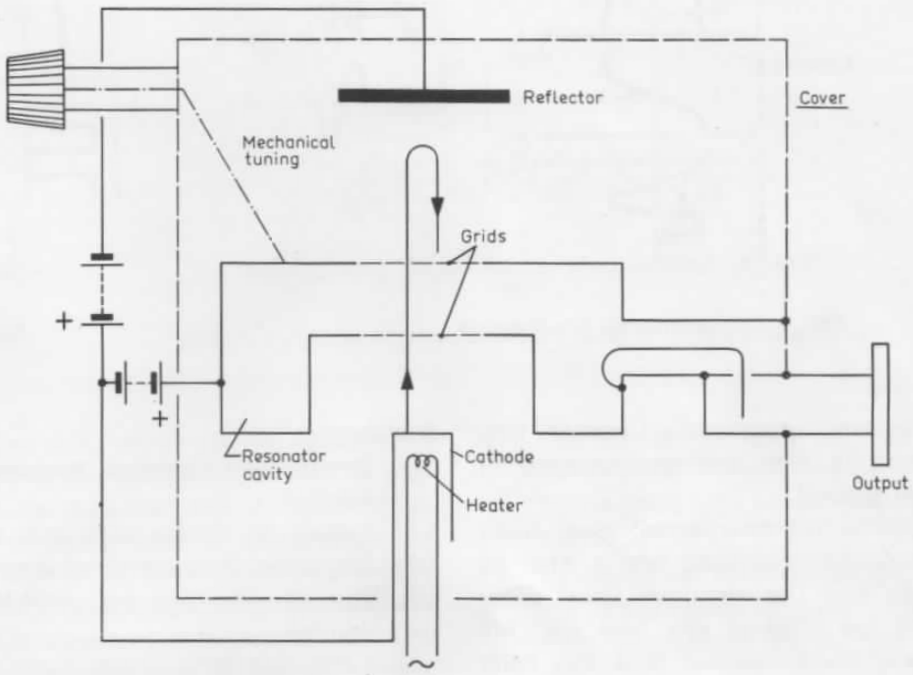
\includegraphics[width=0.85\textwidth]{figure/reflex-klystron.png}
    \caption{Schematische Darstellung eines Reflex-Klystrons.\cite{V53}}
    \label{fig:reflexklystron}
\end{figure}

Elektronen treten aufgrund des Edison-Effektes aus einem Glühdraht aus und werden von den zwei positiv geladenen Gittern des Resonators in Richtung des Reflektors beschleunigt.
Der Reflektor selbst ist jedoch negativ geladen, sodass die Elektronen von ihm zurück in Richtung des Resonators gestoßen werden.
Dies führt zu einem Schwingen des Klystrons.
Die Elektronen werden stets beschleunigt oder abgebremst.
Die Beeinflussung der Elektronengeschwindigkeit wird auch Geschwindigkeitsmodulation genannt.
Aufgrund der unterschiedlichen Geschwindigkeiten bilden sich im Resonator Elektronenbündel aus, die zwischen den Gittern des Resonators in Wechselwirkung mit dem elektrischen Feld treten.
Je nach Zeitpunkt des Eintreffens entziehen sie dem Resonator Energie oder geben Energie an ihn ab, was zur Entstehung von Mikrowellenstrahlung führt.

